\documentclass{article}
\usepackage{graphicx} % Required for inserting images
\usepackage[french]{babel}
\usepackage[T1]{fontenc}
\usepackage[utf8]{inputenc}
\usepackage{amsmath}
\usepackage{txfonts}
\usepackage{color}
\usepackage{url}
\usepackage{ulem}
\usepackage{caption}
\usepackage{subcaption}
\usepackage{tgpagella}

\usepackage{geometry}
\geometry{
  a4paper,
  margin=25.4mm
}

\usepackage{lmodern,mathrsfs}
\usepackage{xparse}
\usepackage[inline,shortlabels]{enumitem}
\usepackage[most]{tcolorbox}
\tcbuselibrary{minted} % tcolorbox minted library, required to use the "minted" tcb listing engine (this library is not loaded by the option [most])
\usepackage{minted} % Allows input of raw code, such as Python code
\usepackage[colorlinks=true, linkcolor=blue, citecolor=green, urlcolor=cyan]{hyperref}

% Custom tcolorbox style for Python code (not the code or the box it appears in, just the options for the box)
\tcbset{
    pythoncodebox/.style={
        enhanced jigsaw,breakable,
        colback=gray!10,colframe=gray!20!black,
        boxrule=1pt,top=2pt,bottom=2pt,left=2pt,right=2pt,
        sharp corners,before skip=10pt,after skip=10pt,
        attach boxed title to top left,
        boxed title style={empty,
            top=0pt,bottom=0pt,left=2pt,right=2pt,
            interior code={\fill[fill=tcbcolframe] (frame.south west)
                --([yshift=-4pt]frame.north west)
                to[out=90,in=180] ([xshift=4pt]frame.north west)
                --([xshift=-8pt]frame.north east)
                to[out=0,in=180] ([xshift=16pt]frame.south east)
                --cycle;
            }
        },
        title={#1}, % Argument of pythoncodebox specifies the title
        fonttitle=\sffamily\bfseries
    },
    pythoncodebox/.default={}, % Default is No title
    %%% Starred version has no frame %%%
    pythoncodebox*/.style={
        enhanced jigsaw,breakable,
        colback=gray!10,coltitle=gray!20!black,colbacktitle=tcbcolback,
        frame hidden,
        top=2pt,bottom=2pt,left=2pt,right=2pt,
        sharp corners,before skip=10pt,after skip=10pt,
        attach boxed title to top text left={yshift=-1mm},
        boxed title style={empty,
            top=0pt,bottom=0pt,left=2pt,right=2pt,
            interior code={\fill[fill=tcbcolback] (interior.south west)
                --([yshift=-4pt]interior.north west)
                to[out=90,in=180] ([xshift=4pt]interior.north west)
                --([xshift=-8pt]interior.north east)
                to[out=0,in=180] ([xshift=16pt]interior.south east)
                --cycle;
            }
        },
        title={#1}, % Argument of pythoncodebox specifies the title
        fonttitle=\sffamily\bfseries
    },
    pythoncodebox*/.default={}, % Default is No title
}

% Custom tcolorbox for Python code (not the code itself, just the box it appears in)
\newtcolorbox{pythonbox}[1][]{pythoncodebox=#1}
\newtcolorbox{pythonbox*}[1][]{pythoncodebox*=#1} % Starred version has no frame

% Custom minted environment for Python code, NOT using tcolorbox
\newminted{python}{autogobble,breaklines,mathescape}

% Custom tcblisting environment for Python code, using the "minted" tcb listing engine
% Adapted from https://tex.stackexchange.com/a/402096
\NewTCBListing{python}{ !O{} !D(){} !G{} }{
    listing engine=minted,
    listing only,
    pythoncodebox={#1}, % First argument specifies the title (if any)
    minted language=python,
    minted options/.expanded={
        autogobble,breaklines,mathescape,
        #2 % Second argument, delimited by (), denotes options for the minted environment
    },
    #3 % Third argument, delimited by {}, denotes options for the tcolorbox
}

%%% Starred version has no frame %%%
\NewTCBListing{python*}{ !O{} !D(){} !G{} }{
    listing engine=minted,
    listing only,
    pythoncodebox*={#1}, % First argument specifies the title (if any)
    minted language=python,
    minted options/.expanded={
        autogobble,breaklines,mathescape,
        #2 % Second argument, delimited by (), denotes options for the minted environment
    },
    #3 % Third argument, delimited by {}, denotes options for the tcolorbox
}

\title{Rapport de Laboratoire - Control Theory}
\author{Nicolas Juruet (21211) - Xavier Allaud(21151)}
\date{March 2024}

\begin{document}

\maketitle

\section{Introduction}
Le but de ce rapport est d'expliquer le processus de conception d'un régulateur PID avec une boucle de rétroaction en utilisant un kit TCLab. Pour se faire, il faudra identier la dyamique d'entrée/sortie du système afin de construire un modèle de celui-ci. Sur base de ce modèle, il sera possible d'implémenter un PID discret qu'il faudra ensuite optimiser puis tester en conditions réelles.
\tableofcontents

\newpage

\section{Identification de la Dynamique du Processus}
\subsection{Graphique}
Application d'un step $X(s) = \frac{1}{s}$ lorsque le système se situe en régime établi pour analyser la ``step response'' $Y(s) = \frac{P(s)}{s}$iiiii.
\begin{figure}[h]
    \centering
    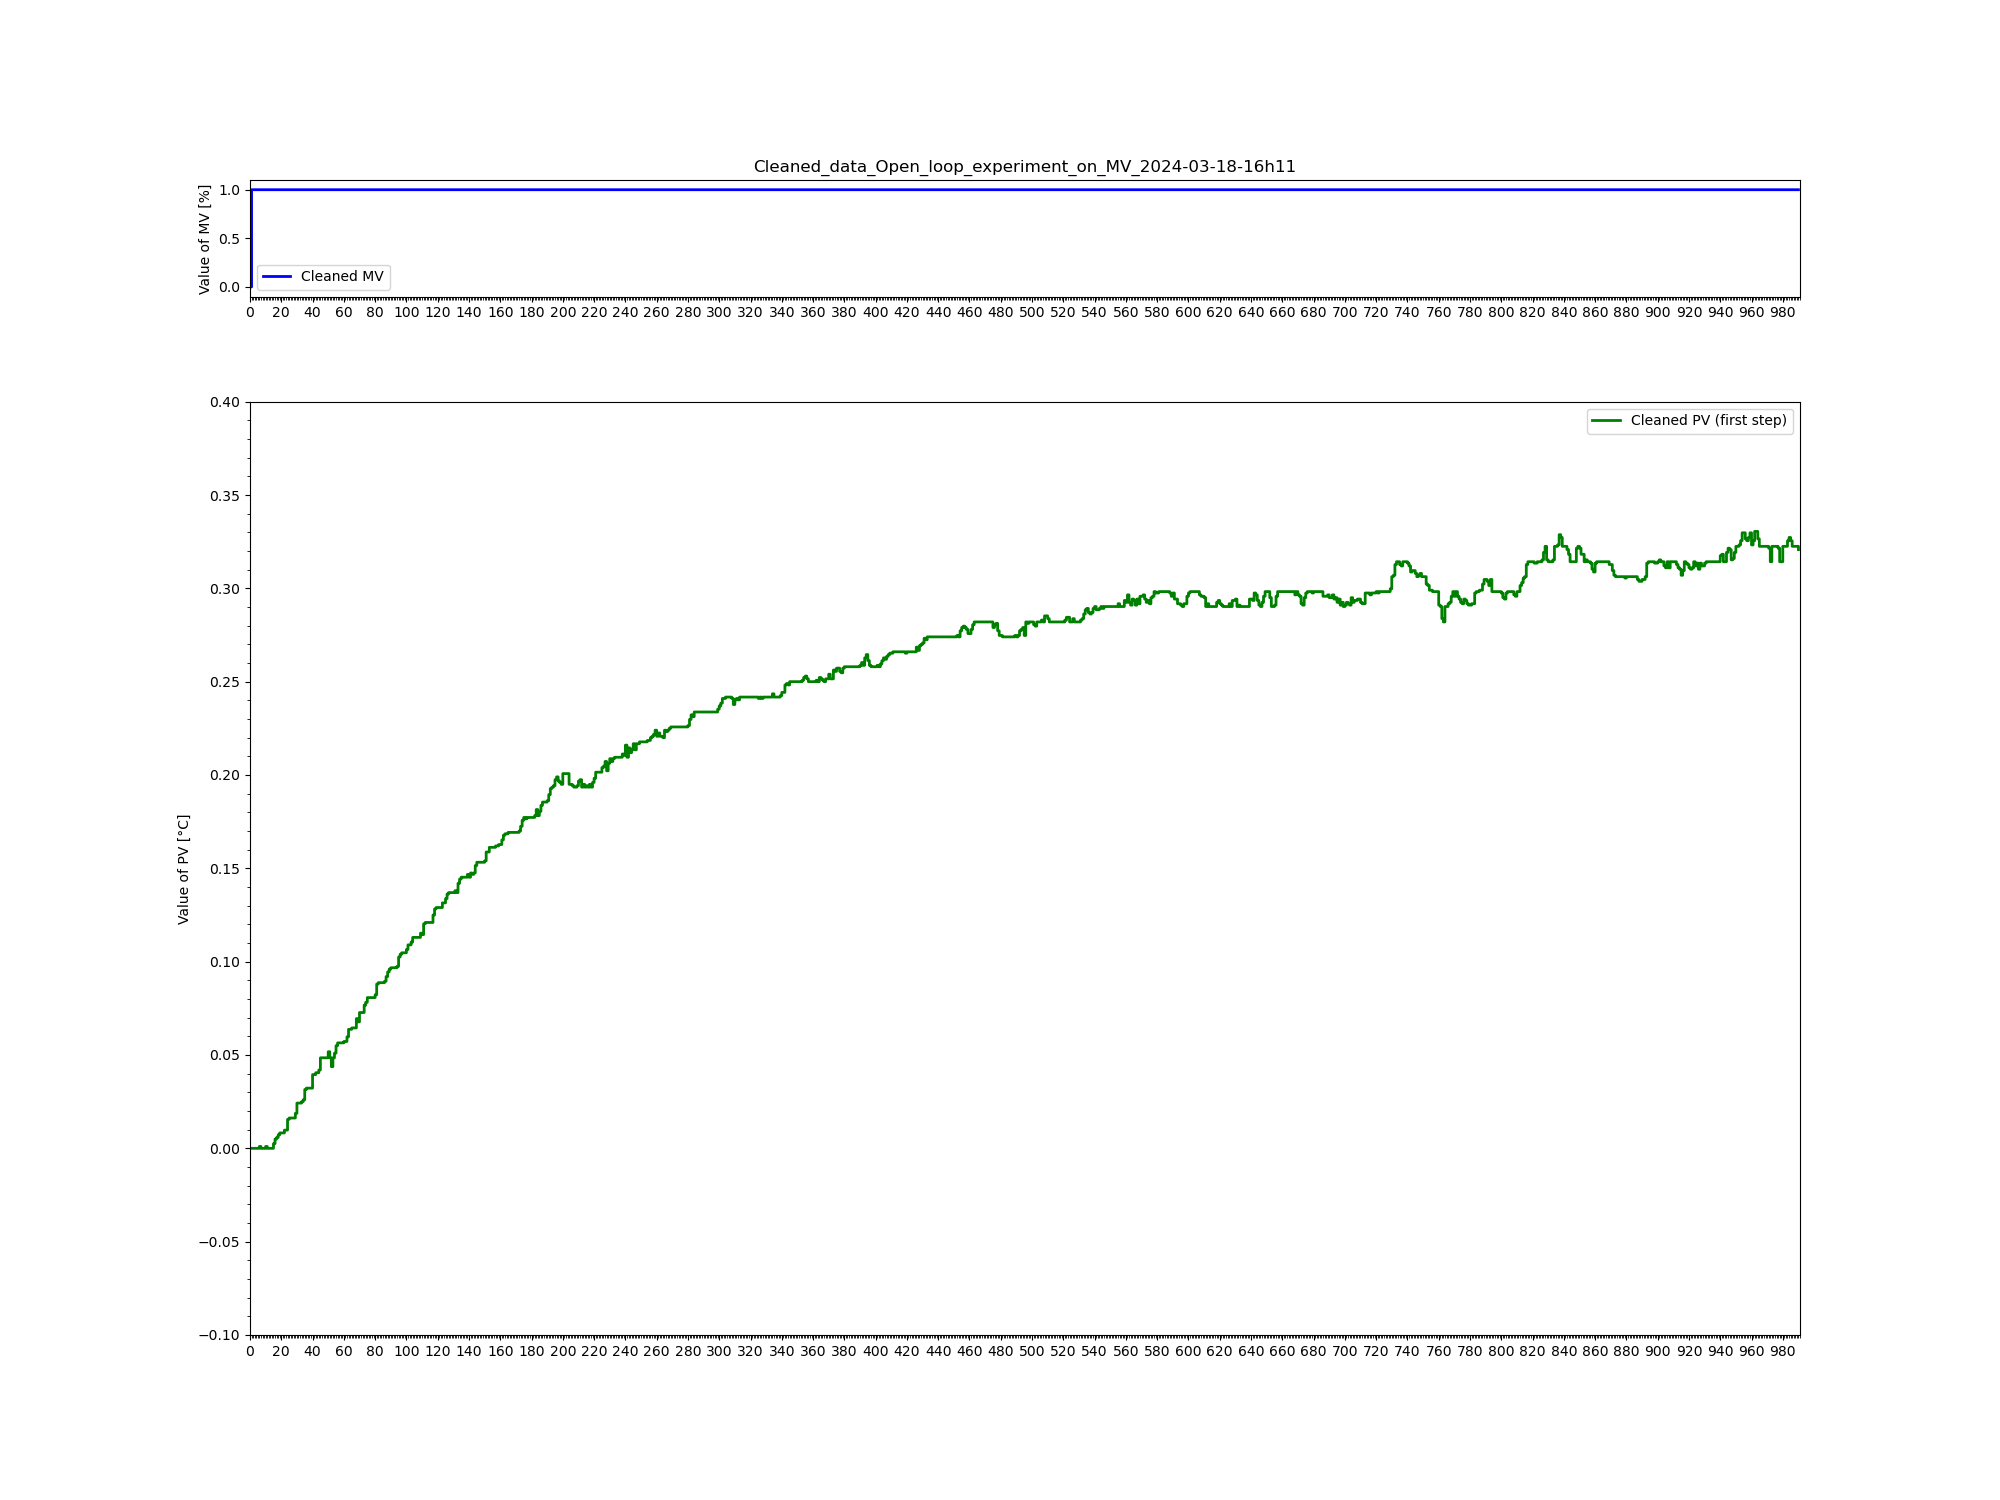
\includegraphics[width=0.9\textwidth]{../Plots/Graphical_methods_Cleaned_data_Open_loop_experiment_on_MV_2024-03-18-16h11.png}
    \caption{Graphique step response}
    \label{fig:Graph1}
\end{figure}
\begin{enumerate}
    \item Le graphique (\ref{fig:Graph1}) obtenu permet (presque) d'affirmer que le processus est un système du $1^{e}$ ordre avec un délai. L'allure de la ``step response" est donc $y(t) = K_p (1-e^{-t/T})u(t)$.

    \item Le but est maintenant d'obtenir les paramètres de la fonction de transfert du processus $P(s)$ ce qui permettra de prédire $Y(s)$ pour n'importe quel $X(s)$ puisque $Y(s) = P(s) \cdot X(s)$ ou $PV = P(s)\cdot MV$. 
    \\Pour se faire, on utilise une fonction de minimisation d'erreur : 
    \begin{python*}
        minimize(FOPDT_cost,
            p0,args=(MVm,PVm,Ts,
            (fig,ax1,l1,l2)), 
            method='Powell',
            bounds=bnds,
            options={'maxiter': maxIter})
    \end{python*}

    Où \texttt{p0} contient les points de départ d'optimisation pour les paramètres \texttt{Kp, T} et \texttt{theta}. La fonction de minimisation va faire varier ces paramètres afin que la fonction de coût, \texttt{FOPDT\_cost}, renvoie la valeur la plus basse possible. 
    \\ \texttt{FOPDT\_cost} : 

    \begin{python*}
        for i in range(0,len(MV)):
            t.append(i*Ts) #calcule le temps correspondant au point actuel                  de la donnée en se basant sur la période de sample
            MVTemp.append(MV[i]) #itère sur la longueur du vecteur d'entrée

            Delay_RT(MVTemp,theta,Ts,MVDelay) #application d'un délai à MV  
            FO_RT(MVDelay,Kp,T,Ts,PVSim) #On applique un délai au premier ordre via le délai appliqué à MV puis on calcule un point du vecteur de sortie à chaque itération 
            objective = objective + (PV[i] - PVSim[i])**2 #on ajoute le carré de l'erreur actuel à la somme des carré des erreurs précédentes   
    \end{python*}
\end{enumerate}

    

\end{document}